\documentclass{article}

% if you need to pass options to natbib, use, e.g.:
% \PassOptionsToPackage{numbers, compress}{natbib}
% before loading nips_2017
%
% to avoid loading the natbib package, add option nonatbib:
% \usepackage[nonatbib]{nips_2017}

%\usepackage{nips_2017}

% to compile a camera-ready version, add the [final] option, e.g.:
\usepackage[final]{nips_2017}

\usepackage[utf8]{inputenc} % allow utf-8 input
\usepackage[T1]{fontenc}    % use 8-bit T1 fonts
%\usepackage{hyperref}       % hyperlinks
\usepackage{url}            % simple URL typesetting
\usepackage{booktabs}       % professional-quality tables
\usepackage{amsfonts}       % blackboard math symbols
\usepackage{nicefrac}       % compact symbols for 1/2, etc.
\usepackage{microtype}      % microtypography
\usepackage{tikz}
\usetikzlibrary{shapes,arrows}

\title{Object Classification using Local Feature Learning of Raw LiDAR Point Clouds}

% The \author macro works with any number of authors. There are two
% commands used to separate the names and addresses of multiple
% authors: \And and \AND.
%
% Using \And between authors leaves it to LaTeX to determine where to
% break the lines. Using \AND forces a line break at that point. So,
% if LaTeX puts 3 of 4 authors names on the first line, and the last
% on the second line, try using \AND instead of \And before the third
% author name.

\author{
  Nikhil Nakhate \\
  Department of Computer Science\\
  University of Wisconsin-Madison\\
  Madison, WI 53706\\
  \texttt{nakhate@wisc.edu} \\
  %% examples of more authors
  \And
  Kamini Jodha \\
  Department of Electrical and Computer Engineering\\
  University of Wisconsin-Madison\\
  Madison, WI 53706\\
  \texttt{jodha@wisc.edu} \\
  %%
  \AND
  Asher Elmquist \\
  Department of Mechanical Engineering\\
  University of Wisconsin-Madison\\
  Madison, WI 53706\\
  \texttt{amelmquist@wisc.edu} \\
}

\begin{document}

% \nipsfinalcopy is no longer used

\maketitle

\begin{abstract}
  Accurate detection of objects in 3D point clouds is a central problem in many applications, such as autonomous navigation, housekeeping robots, and augmented/virtual reality. In this work, we remove the need of manual feature engineering for 3D point clouds by creating a local feature encoding of neighboring points and then passing it through a ConvNet for detecting objects. Both the feature encoding layers and the detection layers are learned end-to-end. The 3D space of point clouds is divided into fixed sized smaller voxels and points in each voxel are encoded and their features are learned. Furthermore, our network learns an effective discriminative representation of objects with various geometries.
\end{abstract}

\section{Introduction}
Processing LiDAR point cloud data is considered to be the cornerstone of fully autonomous cars. There are multiple sensors present on the car, but LiDAR is considered to be the most critical if our target is level 5 autonomy [3]. Even though the LiDAR perception models used in practice today aren’t robust enough, LiDAR proves to be a key sensor. If we can actually achieve mAP values comparable to Deep ConvNets for images today, using just LiDAR point clouds, we would be one step closer to fully autonomous vehicles being a reality. This work focuses on first constructing local feature encodings of LiDAR points and then training the encoded local features using a Deep ConvNet for classification into object labels.

\section{Dataset}
For this machine learning application, two datasets, a depth map and a point cloud, representing LiDAR data were used. Each dataset used was generated in a simulation environment called Chrono. By using a simulation environment, the setup can easily be changed to produce more training and evaluation samples with known configurations and labels. In the simulation, a virtual LiDAR, was placed at the origin of the world with a flat wall placed 4.5 m away. An object (unit cube or unit sphere) was then placed at a random position and orientation between the lidar and the wall. This data was then saved and a new configuration was generated. For the point cloud data, each point the LiDAR detected is saved, and for the depth map, only the distance obtained by the LiDAR is saved. The LiDAR was setup with 50x50 samples with a field of view of 45 degrees in the vertical and horizontal axes. 

\section{Related Work}
We briefly review related work on 3D object detection from point clouds, images and multimodal fusion methods.

\subsection{3D Object Detection in Point Cloud}

Most of the work for 3D object detection uses handcrafted features of point cloud towards specific tasks[2]. And since it is task specific, it is not trivial to find the optimal feature combination. Other algorithms investigate volumetric and multi-view representation of point cloud for 3D object classification[4,5]. However, volumetric representation is constrained by its resolution due to data sparsity and computation cost of 3D convolution and so it’s challenging to process very large point clouds[4]. Multiview representation render 3D point cloud or shapes into 2D images and then apply 2D ConvNet to classify them. Feature based DNNs convert 3D data to a vector, extract shape features and classify them using FCN. Region proposal network (RPN) is a highly optimized algorithm for efficient object detection. However, this approach requires data to be dense and organized in a tensor structure (e.g. image, video) which is not the case for typical LiDAR point clouds.

\subsection{3D Object Detection in Images}

Image based methods typically involve generation of a 3D model from a set of 2D images and rendering of these models. Given that images provide detailed texture information, many algorithms inferred the 3D bounding boxes from 2D images, the accuracy of image-based 3D detection approaches are bounded by the accuracy of the depth estimation. A breakthrough in recognition and detection tasks on images was due to moving from hand-crafted features to machine-learned features.

\subsection{Multimodal Fusion}

Sensor fusion for robust object detection in changing environments is at the core of many applications in robotics[6]. Combining multiple complementary feature representations is often effective to improve classification. Multiple kernel learning is a popular approach to estimate more complex features.


\section{Algorithm and Implementation}
We tried a variety of approaches before zeroing down on our algorithm[1]. We initially represented the list of points got from the simulation and constructed a big cube where the values were just 1 or 0 representing the presence or absence of a point at that coordinate. We shifted the origin and scaled the point coordinates so that they are positive integers. Reshaping them into smaller voxels and finding non zero elements would then ideally give us the complete local address as to which voxel it is in and where it is present within the voxel. Tensorflow does not allow us to find indices of elements represented in a space that is more than 5 dimensions. So, we manually calculated the local means by mapping the 3 dimensions into a grid dimension (eq. \ref{eq:localcoord}) and local voxel dimension (eq. \ref{eq:voxelcoord}). This was done by using the following formulae:

\begin{equation} \label{eq:voxelcoord}
(x_v, y_v, z_v) = (x, y, z) / (Dv_x, Dv_y, Dv_z)
\end{equation}

In eq. \ref{eq:voxelcoord} above, \(x_v, y_v, z_v\) denote the coordinate of the voxel that point \(x, y, z\) is located within, and \(Dv\) represents the dimensions (depth,width,height) of the voxels.

\begin{equation} \label{eq:localcoord}
(x_i, y_i, z_i) = (x, y, z) \% (Dv_x, Dv_y, Dv_z)
\end{equation}

In eq. \ref{eq:localcoord} above, \(x_i, y_i, z_i\) denote the local coordinate of the point \(x, y, z\) within its voxel. \(Dv\) represents the dimensions (depth,width,height) of the voxels. 

We then used the following formula to index the voxels. This not only gave us the local coordinates of each point but also a hashmap like representation that was used later to make sure each point in every voxel was considered.

\begin{equation} \label{eq:voxel_id}
VoxelID = z_v + y_v*gD_z + x_v*gD_z*gD_x
\end{equation}

( \(gD_x, gD_y,gD_z\) are the dimensions of the grid of voxels.) In eq. \ref{eq:voxel_id} above, the \(VoxeID\) describes which voxel is being considered while only using a single value. With this equation, we can effectively flatten out the voxels and reorder as necessary as each \(VoxelID\) is unique. 

The algorithm chosen predominantly has 3 main parts:\\
\hangindent=0.5cm i)\hspace{.4cm}Dimensionality reduction\\
ii)\hspace{.3cm}Complex local feature learning\\
iii)\hspace{.2cm}Object detection by learning global feature maps

\subsection{Dimensionality Reduction}

LiDAR point clouds are generally sparse. Also given a particular LiDAR point cloud, the distribution is non-uniform. If a point cloud is used directly in a ConvNet using 3D convolutions, not only that the computational time increases manifold, there is also a very high chance of overfitting the dataset. We thus fix the number of points that are at most chosen at random from each voxel to 30 (let us call this m). 

\begin{figure}
	\centering
	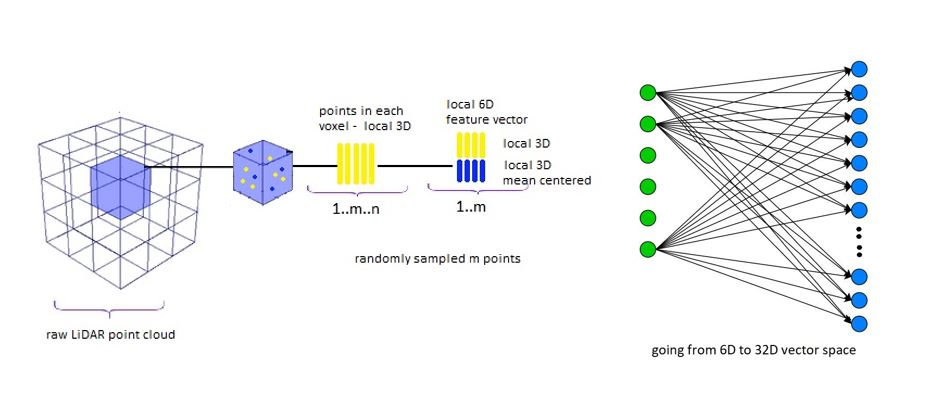
\includegraphics[width=1.0\textwidth]{Final_figure.jpg}
	\caption{Visual depiction of our neural network referenced in this paper.}
\end{figure}

\subsection{Complex local feature learning}

Local features viz local coordinates of points + local mean centred coordinated (resulting 6D feature vector) are mapped into a higher dimensional feature space (32 dimensions) so that it can learn complex local features. This is done by mimicking the behavior of a fully connected network. The key point here is since it would be extremely inconvenient to have a fully connected layer for each voxel separately, we flatten it. But we have to make sure that only local features are encoded. The actual implementation was done by flattening the voxel into a 3D matrix of size \((m*gD_x*gD_y*gD_z) \times 1 \times (padzero + 6 + padzero) \) (where \(gD_x\), \(gD_y\), and \(gD_z\) are the dimensions of the grid of voxels). We add padding in the depth dimension to the front and back of the matrix. We use a filter kernel of size \((m*gD_x*gD_y*gD_z) \times 1 \times 32 \).

\subsection{Object detection by learning global feature maps}
The feature vectors are then reshaped to bring the original neighboring voxels closer to each other to allow for inter-voxel learning at the start of the global feature learning portion of the neural network. This last part involves learning global feature maps using convolution layers so that the network can understand how the various local features interact with each other. We use two alternating convolution and maximum pooling layers followed by a dense layer and output through a softmax layer. 

The above neural network was implemented in tensorflow.

\section{Discussion of Results}
Consider our architecture as divided into 4 blocks. We remove each block and point out the importance of each block in this section:

%\tikzstyle{decision} = [diamond, draw, fill=blue!20, 
%text width=4.5em, text badly centered, node distance=3cm, inner sep=0pt]
\tikzstyle{block} = [rectangle, draw, fill=blue!20,node distance=3.5cm, 
text width=5em, text centered, rounded corners, minimum width=3cm, minimum height=2em]
\tikzstyle{line} = [draw, -latex']
%\tikzstyle{cloud} = [draw, ellipse,fill=red!20, node distance=3cm,
%minimum height=2em]

\begin{tikzpicture}[node distance = 2cm, auto]
% Place nodes
\node [block] (data) {Data: Depth map or point cloud};
\node [block, right of=data] (6d) {Local Feature Vector};
\node [block, right of=6d] (features) {Higher Dimensional Feature Vector};
\node [block, right of=features] (connected) {Fully Connected Layers for Detection and Classification};

%\node [cloud, left of=init] (expert) {expert};
%\node [cloud, right of=init] (system) {system};
%\node [block, below of=init] (identify) {identify candidate models};
%\node [block, below of=identify] (evaluate) {evaluate candidate models};
%\node [block, left of=evaluate, node distance=3cm] (update) {update model};
%\node [decision, below of=evaluate] (decide) {is best candidate better?};
%\node [block, below of=decide, node distance=3cm] (stop) {stop};
% Draw edges
\path [line] (data) -- (6d);
\path [line] (6d) -- (features);
\path [line] (features) -- (connected);
%\path [line] (decide) -| node [near start] {yes} (update);
%\path [line] (update) |- (identify);
%\path [line] (decide) -- node {no}(stop);
%\path [line,dashed] (expert) -- (init);
%\path [line,dashed] (system) -- (init);
%\path [line,dashed] (system) |- (evaluate);
\end{tikzpicture}

The training data used for all the different architectures considered in this work is a set of 1000 equally distributed and randomly shuffled samples for the point cloud network, and 3000 equally distributed and randomly shuffled samples for the depth map. The test data used is 500 equally distributed samples for the point cloud network, and 1000 for the depth map. The difference in samples between depth map and point cloud networks is due to the additional computation required for the higher dimensional feature vector learning layer. The learning rate used is also maintained at a constant value: 0.001. We have fixed these parameters so that we get an interpretable comparison of all the architectures considered.

Using a bare minimum network configuration of just a depth map of points representing a 3D space using a 2D matrix with values of depth for each element. We pass this 2D matrix through the ConvNet and calculate the accuracy. We get a test accuracy of about \textbf{57\%} in this case. The reasons for this low accuracy are two-fold. Since we are reducing one dimension and projecting on a 2D plane, some amount of information is lost right about locality. Secondly, since we have a sparse set of points and the convolution layers are not optimized to handle sparsity, the neural net has a hard time localizing the image. A better approach for training using a depth map is by using bounding boxes for object and using the object position and orientation as labels. We can bypass the localization problem using local feature encodings as we see in the other architectures.

We then add a 3D to 6D local feature vector layer. This first converts the 3D coordinates of the points in the entire space considered to a local set of 3D coordinates per voxel. We then create a 6D feature vector by appending the 3D coordinates to the mean centered 3D coordinates of the same points. With this architecture, we get an accuracy of about \textbf{88\%}.

We then add another layer to map the 6D vector representation of points to a higher dimensional feature space so that complex local features for compound shapes can be learnt. For example, consider a voxel containing a part of a sphere. We would need to map each local feature to a higher dimension so that it actually learns how to identify the spherical sector. Using this architecture, we get an accuracy of about \textbf{91\%}. We would typically expect a bigger jump in accuracy from the previous method if more number of complex shapes were used. But since we have used only two shapes namely a cube and a sphere (both of which are regular shapes and only the sphere being curvilinear) the jump in the accuracy isn’t significant.



\section{Conclusion}
Traditional ConvNet architectures use only RGB images to detect objects from the scene. True depth information is never used by the network for detection or deciphering shape information. The only two ways for the neural network to work with true depth information is using raw LiDAR points or using a depth map and running it through a ConvNet. Empirically adding local feature encoding layers works better than running a depth map through a ConvNet.

\section{Future Work}
We would like to test the performance on real world data. Currently we are only using simulated data. Since it generated from the simulator, we cannot account for noise resulting from ambient illumination, different surface properties, interreflections etc. We would also want to consider irregular or compound shapes and compare the corresponding results on the neural network that takes a depth map as an input.

We also hope to consider many more object classes and have another object detection metric for the comparison of ConvNet architectures like mAP. Needless to say that we would also have another set of labels to actually measure these metrics in addition to the object class label which would be orientation of the object in space and position of object. This would then be a multi-task learning problem and would be able to achieve the full potential of learning from the data.  


\section*{References}

[1] Yin Zhou, Oncel Tuzel, Apple Inc. VoxelNet: End-to-End Learning for Point Cloud Based 3D Object Detection

[2] H. Ling and D. W. Jacobs. Shape classification using the inner-distance. {\it IEEE transactions on pattern analysis and machine intelligence.}

[3] Barbara Wendling, Chair, J3016 Task Force. First Revision of J3016- Update on Task Force Activities

[4] A. Gonzalez, D. Vazquez, A. Lopez, and J. Amores. Onboard object detection: Multicue, multimodal, and multiview random forest of local experts. {\it IEEE Transactions on Cybernetics}, 2016

[5] Charles R. Qi, Hao Su, Kaichun Mo Leonidas J. Guibas Stanford University. PointNet: Deep Learning on Point Sets for 3D Classification and Segmentation

[6] Oier Mees, Andreas Eitel, Wolfram Burgard. Choosing Smartly: Adaptive Multimodal Fusion for Object Detection in Changing Environments




%
%[1] Alexander, J.A.\ \& Mozer, M.C.\ (1995) Template-based algorithms
%for connectionist rule extraction. In G.\ Tesauro, D.S.\ Touretzky and
%T.K.\ Leen (eds.), {\it Advances in Neural Information Processing
%  Systems 7}, pp.\ 609--616. Cambridge, MA: MIT Press.
%
%[2] Bower, J.M.\ \& Beeman, D.\ (1995) {\it The Book of GENESIS:
%  Exploring Realistic Neural Models with the GEneral NEural SImulation
%  System.}  New York: TELOS/Springer--Verlag.
%
%[3] Hasselmo, M.E., Schnell, E.\ \& Barkai, E.\ (1995) Dynamics of
%learning and recall at excitatory recurrent synapses and cholinergic
%modulation in rat hippocampal region CA3. {\it Journal of
%  Neuroscience} {\bf 15}(7):5249-5262.

\end{document}